\documentclass[a4paper, 12pt]{article}
\usepackage{cite}
\usepackage{multicol, caption}
\usepackage{titling}
\usepackage{graphicx}
\usepackage{tabularx}
\usepackage{subcaption}
\usepackage{url}
\newenvironment{Figure}
  {\par\medskip\noindent\minipage{\linewidth}}
  {\endminipage\par\medskip}

%加這個就可以設定字體
\usepackage{fontspec}
%使用xeCJK,其他的還有CJK或是xCJK
\usepackage{xeCJK}
\usepackage[margin=0.6in]{geometry}

%字型的設定可以使用系統內的字型,而不用像以前一樣另外安裝
\setCJKmainfont{DFKai-SB}
\author{}    
\newcommand*{\citenumfont}{}

% Reducing Distance of title and date
\setlength{\droptitle}{-2cm}
\title{\textbf{Fake News Classification}}
\renewcommand\maketitlehookc{\vspace{-3.5em}}


\begin{document}
    \maketitle     
    \begin{center}
        \begin{tabular}{ccc}
            陳君彥, b04703091 & 陳柔安, b04701232 & 蕭法宣, b04705007 \\
            b04703091@ntu.edu.tw &
            b04701232@ntu.edu.tw &
            b04705007@ntu.edu.tw
        \end{tabular}
    \end{center}

    \begin{figure}[h!]
        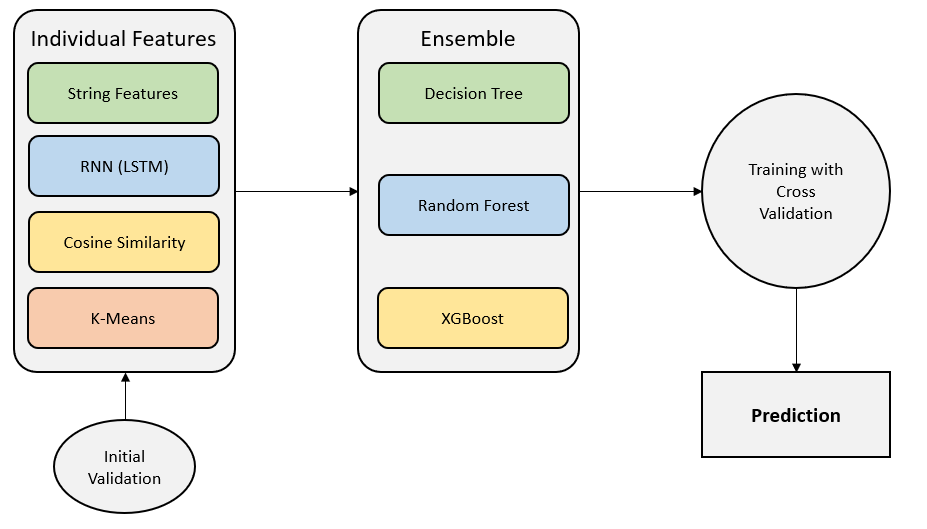
\includegraphics[width=\linewidth]{images/outline.png}
        \caption{Outline of our prediction method. Extracting useful features of the dataset and ensembled with 3 different aggregation methods. Final model is trained and chosen with cross validation and applied onto the testing data set to make our final prediction.}
        \label{outline}
    \end{figure}

    \section*{Division of Work}
        陳君彥, b04703091: 
        \begin{itemize}
            \item Generation and testing of embedding based features.
            \item Generation and testing of k-means embedding model.
            \item Creation of written report.
        \end{itemize}
        陳柔安, b04701232:
        \begin{itemize}
            \item Creation of ensemble method scripts.
            \item Further testing of RNN models.
            \item Testing and submission of final prediction.
        \end{itemize}
        蕭法宣, b04705007:
        \begin{itemize}
            \item Initial testing of RNN models.
            \item Generation and testing of string based features.
            \item Code project cleanup and sorting.
        \end{itemize}

    \begin{multicols}{2}
        \section{Introduction}
            The goal of the WSDM 2019 Fake News Classification \cite{wsdm} challenge is to indentify and tags pairs of news title on whether the two titles are 'unrelated' to each other, 'agreed' with each other, or 'disagreed' with each other. The data is given in simplified chinese, with machine translated english version. The first title of the pair was a known 'fake news' article, and so the challenge could lend a hand in identifying misinformation in the real world.

            \begin{center}
                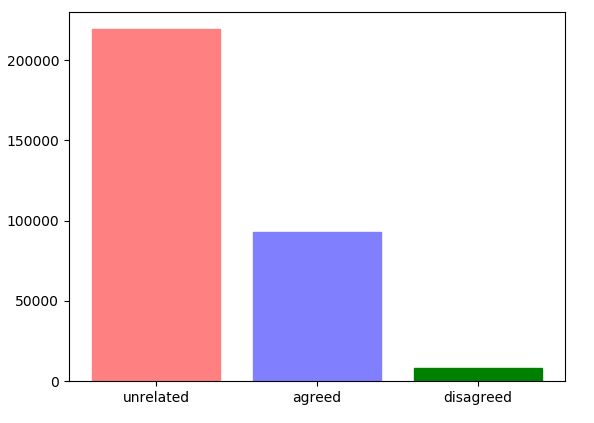
\includegraphics[width=\linewidth]{images/label_dist.png}
                \captionof{figure}{The occurence of each label in the training data set}
                \label{label_dist}
            \end{center}
            \vskip 0.2cm

            The data is distributed as shown in Figure \ref{label_dist}, with unrelated holding the majority, and with very little data labeled disagree. This proved problematic as it tended to push our models to predict a label as unrelated. Even with the challenge's given weights of 1/16, 1/15, 1/5 for scoring, it still struggled to make a visible difference.

        \section{Method}
            We approached this problem as summarized in Figure \ref{outline}, first by attempting to extract meaningful features in our dataset, testing each individual features, and then combining them in ensemble machine learnin methods to create our final strong prediction. We used cross validation to pick our final trained model, with drop-out and early stopping for regularization.
        
            \subsection{Preprocessing}
            Our dataset is given to us with the titles uncut in chinese, as well as a machine translated english version of the title. As the machine translated version is not fully accurate, we performed most of our analysis on the chinese titles.

            \paragraph*{Tokenization} The chinese titles were cut with jieba \cite{jieba} with stopwords removed, and the english titles were cut with nltk.word\_tokenize \cite{nltk}, with case removed and contractions expanded.

            \paragraph*{Embedding Model} We trained both a chinese and english embedding model using the gensim.Word2Vec \cite{gensim} using the CBOW embedding model. The training was done on the original training data. The CBOW model uses

        \subsection{Individual Features}
            \subsubsection{String Features}
                \paragraph*{Overlap Ratio, Partial-Overlap Ratio, Tokenset Overlap Ratio} We calculate these three ratios to provide some basic numbers on the similarity between the two titles. These ratios mainly serve to separate titles that are "unrelated" to those that are "related" ("agreed" + "disagreed").

                \paragraph*{"Rumor" Word Count} As the first title in our dataset is always "fake news", we noticed that there are specific "rumor" words that indicate a title is likely to be fake news. Counting the occurence of such words in the second title gives us some indication on whether the second title is also a rumor, lending to us some indications onto whether the titles agree or disagree.
            
            \subsubsection{Embedding Features}
                \paragraph*{Sentence Similarity} With the trained embedding model, we calculated the combined word vectors for each sentence to create a sentence vector, then calculated a sentence similarity score through cosine similarity. This assisted in the differentiation of "related" and "unrelated" titles.

                \paragraph*{Noun Object Distance} With the trained embedding model, we attempt to calculate the distance between nouns of the two titles, as we imagined that the nouns are more likely to be the focus subject of each title. However, due to the poor performance of jieba's POS tagging, we elected to use the english titles, and picked out the nouns using the POS Perceptron Tagger in NLKT. \cite{percTag}

            \subsubsection{K - Means, Transitivity}
                As the classification for each title are wholly individual, we realized that we can obtain transitivity relations between titles. i.e. if Sentence A agrees with Sentence B, and Sentence C disagrees with Sentence A, we can arrive at the conclusion that Sentence B also disagrees with Sentence C. 
                
                Using this property, we tested out a modified k-means model on the sentence vectors acquired through embedding, with the node distances being the cosine similarity of the titles.

        \subsection{Ensemble}
            With the above individual weak features of our models, we tested out the following ensemble methods: Decision Tree, Random Forest, XGBoost, and used the earlier features as the inputs to create our prediction model. Through validation testing, XGBoost performed the best and was chosen as our model for the final submission, reaching.

        \subsection{RNN Models}
            We noticed the high performance of RNN based models from the submissions of other participants, and decided to further test the following models.
            
            \begin{itemize}
                \item LSTM
                \item GRU
                \item LSTM-bidirectional
                \item GRU-bidirectional
                \item LISTM + Word2Vec
                \item Multilayer GRU
            \end{itemize}

            Most notable was the strong overfitting of these models on our dataset, with the in-sample and validation accuracy having a difference of over 10\% on several of the models, even with early dropout. The best performing Multilayer GRU achieved a 75\% validation accuracy, and a 73.5\% accuracy on the submission. 
            
    \section{Experiments}
        Before incorporating each feature into our ensemble model, we individually tested some of the features to see if they were valid features that can be used.
        \subsection{Embedding}
        \begin{Figure}
            \centering
            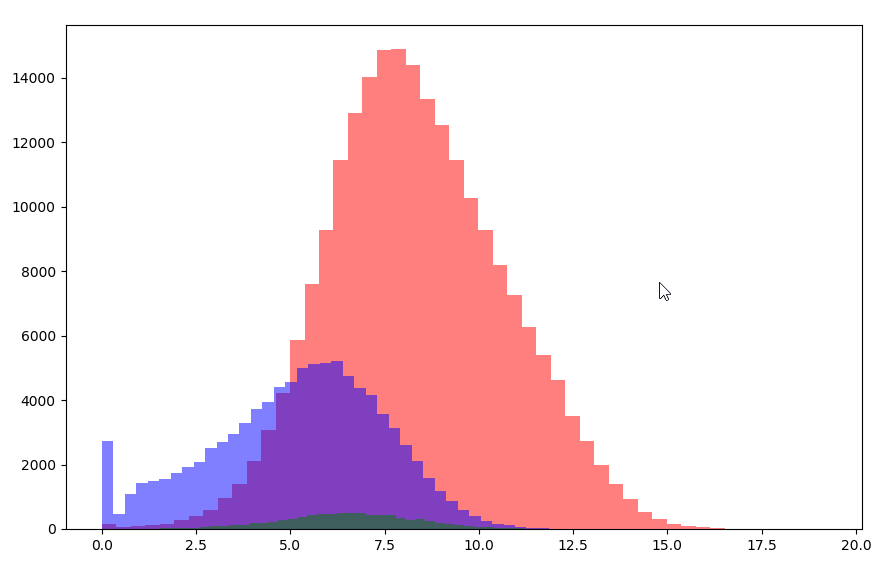
\includegraphics[width=\linewidth]{images/embedding_dist.png}
            \captionof{figure}{Distribution of "agreed" (blue), "disagreed" (green), "unrelated"(red) with regards to sentence similarity distance}
            \label{embed_dist}
        \end{Figure}
        \begin{center}
                \begin{tabular}{ccc}
                    Window & Vocababulary& Accuracy \\
                    \hline
                    2 & 60 & 0.775235 \\
                    2 & 70 & 0.775923 \\
                    2 & 80 & 0.775693 \\
                    \hline
                    5 & 60 & 0.773631 \\
                    5 & 70 & 0.773828 \\
                    5 & 80 & 0.773926 \\
                    \hline
                    10 & 60 & 0.773173 \\
                    10 & 70 & 0.773500 \\
                    10 & 80 & 0.773959 \\
                \end{tabular}
            \captionof{figure}{Finding the best parameters for CBOW model.}
        \end{center}
        
        We tested if sentence similarity could be used as one method to distinguish "unrelated" from "related". This also helped us pick the optimal CBOW parameters. The distribution shows that 'unrelated' follows a different distribution to that of 'related' titles. Using sentence similarity alone we were able to achieve an validation accuracy of 77\%, though this resulted in the model largely guessing 'agreed' for everything else that isn't 'unrelated'. Hence we needed a different method to separate them.
        
    \end{multicols}
        \begin{center}
            \centering
            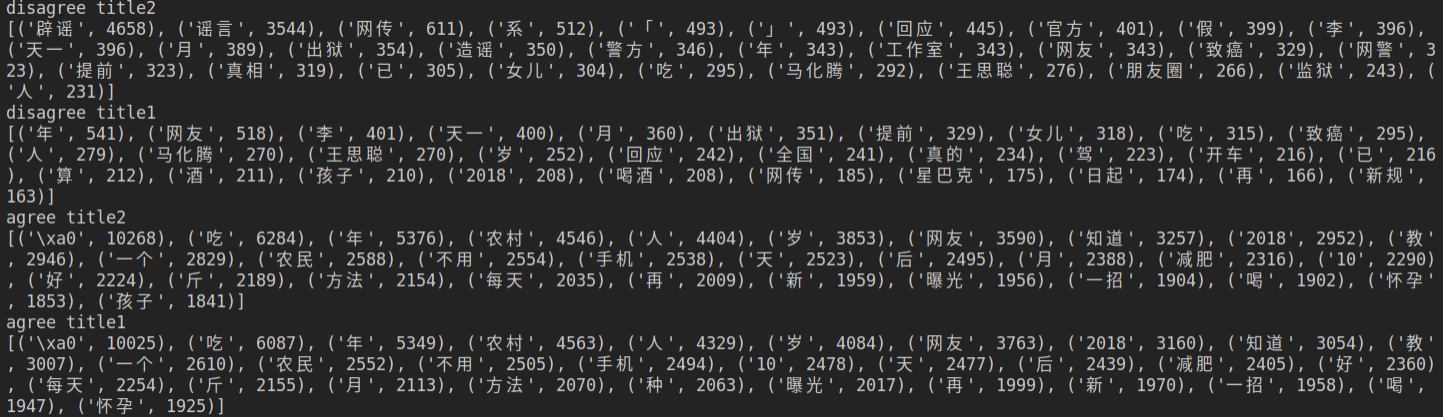
\includegraphics[width=\linewidth]{images/rumor_words.png}
            \captionof{figure}{Occurence of words in titles for different labels}
            \label{rumor}
        \end{center}
    \begin{multicols}{2}

        \subsection{Counting Features}
            As shown in Figure \ref{rumor}, we noticed some specific words that stood out when looking at 'agreed' and 'disagreed'. With some human knowledge, we picked "谣", "官方", "假", "真相" and used their occurence count as a feature. This worked out to be the most important in differentiating between related titles.

        \subsection{Ensemble}
            Our final submission was the aggregation of the previous features, with Figure \ref{ensemb_results} being our final results. We tested the addition of each feature, and measured the change in validation accuracy with each additional feature, as shown in Figure \ref{ensemb_detail}, and with the importance of each feature as shown in Figure \ref{importance}

            \begin{center}
                \begin{tabular}{l|c}
                    New Feature & Validation Accuracy\\
                    \hline
                    String Features & 0.81866 \\
                    + Sentence Similarity & 0.81716 \\
                    + Noun Similarity & 0.81647 \\
                    + K-Means & 0.82034
                \end{tabular}
                \captionof{figure}{Validation Accuracy for each additional feature}
                \label{ensemb_detail}
            \end{center}

            \begin{center}
                \begin{tabular}{l|c}
                    Feature & Importance\\
                    \hline
                    overlap ratio & 0.498709 \\
                    partial ratio & 0.124975 \\
                    tokenset ratio & 0.04927 \\
                    rumor word count & 0.29825 \\
                    sentence similarity & 0.01066 \\
                    noun similarity & 0.00264 \\
                    k-means & 0.015499
                \end{tabular}
                \captionof{figure}{Importance of each feature in final model}
                \label{importance}
            \end{center}

            \begin{center}
                \begin{tabular}{l|cc}
                    Method & Validation & Submission\\
                    \hline
                    Decision Tree & 0.75037 & 0.71961 \\
                    Random Forest & 0.80481 & 0.77659 \\
                    XGBoost & 0.82025 & 0.79398 \\
                \end{tabular}
                \captionof{figure}{Results of the ensemble methods}
                \label{ensemb_results}
            \end{center}

        \subsection{RNN}
            We tested out several different RNN models looking for one that can perform similar or better than our ensemble. While none of the models achieved this, as shown in Figure \ref{rnn_results}, it gave us some additional insight and an idea of what to improve. 
            
            However, due to the lack of computing power and time contrainst, we terminated our experiments here, though we surmise that additional layers, and blending with our XGBoost model, the model could perform with a better accuracy.

            \begin{center}
                \begin{tabular}{l|cc}
                    Model & Validation & Submission \\
                    \hline
                    LSTM & 0.7448 & 0.71403 \\
                    GRU & 0.7498 & 0.71917 \\
                    LSTM-bidirectional & 0.7433 & 0.71546 \\
                    GRU-bidirectional & 0.7402 & 0.70804 \\
                    LSTM + Word2Vec & 0.7506 & 0.71664 \\
                    GRU Multilayer & 0.7742 & 0.73807
                \end{tabular}
                \label{rnn_results}
            \end{center}

        \subsection{Failed - Sentiment}
            We originally intended to include the use of sentiment analysis as a feature. However, upon generating the score, we found out that the scores for the three categories followed almost the exact same distribution, providing absolutely no benefit to our model. We theorize that this is due to the short nature of titles, leading to increased use in "eye catching", "power" words, with little change in sentiment. Combined with the very limit amount of words to extract data from led to all the titles being basically the same.
        
    \end{multicols}
    \newpage
    \section{Conclusion}
        We arrive at the conclusion that the aggregation of different features in our data is an effective method in indentifying and classifying fake news. After discussions with classmates and scouring forums for other people's attempt, we also conclude that this method is also rather efficient. 
        
        Our personal machines were all laptop spec'd machines, running the models within an acceptable time frame, with the results being only slightly lower than much more intensive models, such as BERT, which often require much more powerful hardware, and ran upwards of hours when training the models and predicting the results.

        \vskip 5cm
\bibliography{report}{}
\bibliographystyle{ieeetran}

\end{document}
